\chapter{Implementacija i korisničko sučelje}
		
		
		\section{Korištene tehnologije i alati}
		
			\textbf{\textit{dio 2. revizije}} \\
			
			 \textit{Detaljno navesti sve tehnologije i alate koji su primijenjeni pri izradi dokumentacije i aplikacije. Ukratko ih opisati, te navesti njihovo značenje i mjesto primjene. Za svaki navedeni alat i tehnologiju je potrebno \textbf{navesti internet poveznicu} gdje se mogu preuzeti ili više saznati o njima}.
			

    	
        \begin{longtabu} to \textwidth {|X[6, l+3]|X[25, 1]|X[20, 2]|}
		
    		\hline \multicolumn{3}{|c|}{\textbf{Backend}}	 \\[3pt] \hline
    		\endfirsthead
    		
    		\hline
    		\endlastfoot
    		
    		PostgreSQL & \href{https://www.postgresql.org/}{https://www.postgresql.org/}	& Objektno-relacijska baza podataka 	\\ \hline
    		Java 11 & \href{https://www.oracle.com/technetwork/java/javase/downloads/jdk11-downloads-5066655.html}{https://www.oracle.com} & Programski jezik u kojem je napisan backend dio aplikacije	\\ \hline
    		Java Spring Boot & \href{https://spring.io/projects/spring-boot}{https://spring.io/projects/spring-boot} & Razvojni okvir 	\\ \hline
    		
    		Spring Web MVC  & \href{https://docs.spring.io/spring/docs/current/spring-framework-reference/web.html}{https://docs.spring.io/spring/} & Web framework za rukovanje zahtjevima 	\\ \hline
    		Spring Security  & \href{https://spring.io/projects/spring-security}{https://spring.io/projects/spring-security} & 
Moćan i vrlo prilagodljiv okvir za provjeru autentičnosti i kontrolu pristupa 	\\ \hline

        Lombok  & \href{https://projectlombok.org/}{https://projectlombok.org/} & Java library za pregledniji kod 	\\ \hline
    	\end{longtabu}
			
			

			\eject
			
        \begin{longtabu} to \textwidth {|X[4, l+3]|X[25, l]|X[20, 2]|}
		
    		\hline \multicolumn{3}{|c|}{\textbf{Frontend}}	 \\[3pt] \hline
    		\endfirsthead
    		
    		\hline
    		\endlastfoot
    		
    		React & \href{https://reactjs.org/}{https://reactjs.org/}	& JavaScript library za izgradnju sučelja	\\ \hline
    		Ant Design & \href{https://ant.design/}{https://ant.design/} & Design library sa komponentama za lakšu izgradnju korisničkog sučelja	\\ \hline
    		
    		NPM & \href{https://www.npmjs.com/}{https://www.npmjs.com/} & Upravitelj paketa za programski jezik JavasScript	\\ \hline
    		
    		OpenCage Geocoder & \href{https://opencagedata.com/}{https://opencagedata.com/} & API za dohvaćanje koordinata iz adrese	\\ \hline
    	\end{longtabu}			
			
			
        \begin{longtabu} to \textwidth {|X[4, l+3]|X[25, l]|X[20, 2]|}
		
    		\hline \multicolumn{3}{|c|}{\textbf{Komunikacija}}	 \\[3pt] \hline
    		\endfirsthead
    		
    		\hline
    		\endlastfoot
    		
    		Slack & \href{https://slack.com/intl/en-hr/}{https://slack.com/intl/en-hr/}	& Platforma koju smo koristili za lakšu komunikaciju	\\ \hline
    		Trello & \href{https://trello.com/en}{https://trello.com/en} & Alat koji nam je olakšao zajedniči rad i raspoređivanje  projektnih zadataka	\\ \hline
    	\end{longtabu}
    
        \eject
			
			
			
		
	
		\section{Ispitivanje programskog rješenja}
	
			
			\subsection{Ispitivanje komponenti}
			\textit{Potrebno je provesti ispitivanje jedinica (engl. unit testing) nad razredima koji implementiraju temeljne funkcionalnosti. Razraditi \textbf{minimalno 6 ispitnih slučajeva} u kojima će se ispitati redovni slučajevi, rubni uvjeti te izazivanje pogreške (engl. exception throwing). Poželjno je stvoriti i ispitni slučaj koji koristi funkcionalnosti koje nisu implementirane. Potrebno je priložiti izvorni kôd svih ispitnih slučajeva te prikaz rezultata izvođenja ispita u razvojnom okruženju (prolaz/pad ispita). }
			
			
			
			Da bismo testirali backend, napravili smo dvije vrste testova. JUnit testove za testiranje servisa te integracijske testove koje je najlakše opisati kao automatizirane Postman zahtjeve.
			
			Servisi su testirani na način da ih gledamo kao crne kutije koje za određeni ulaz trebaju odraditi određene akcije ili vratiti određene objekte. Nomenklatura testovi servisa (BandServiceTest) slijedi pravilo given\_when\_then. Naprimjer, ako testiramo metodu naziva createMusician, pretpostavljajuci da on još ne postoji i očekujući da se kreira glazbenik u bazi, naziv testa bio bi 
			noSuchMusician\_
			createMusician\_createAndPersistateMusician().
			
			Pomoću Mockito frameworka u testovima mockamo (oponašamo) ulaze te na taj način kontroliramo ulaze i okolinu metode koju testiramo. Drugim riječima, kada radimo test za neku komponentu ili servis, pretpostavljamo da su svi ulazi dobri i ne zanima nas utjecaj naše komponente na drugu komponentu, već samo direktni izlaz. Na taj način dobivamo testove koji su međusobno nepovezani i koji definiraju željeno ponašanje aplikacije. Ukoliko u daljnjem razvoju neki od razvojnih programera promijeni neko ponašanje koje ima utjecaj na druge komponente, pravilno napisani testovi trebali bi pasti i upozoriti ga da će se njegova promjena propagirati dublje u aplikaciju. Testovi koji su pisani ciljano na pojedine komponente sustava u kontroliranim uvjetima prilikom izvođenja precizno ukazuju na vjerojatan izvor pogreške. Na primjer, ako promijenimo implementaciju kreiranja glazbenika te on u trenutku kreiranja ne dobije id, samo testovi koji provjeravaju parametre nakon inicijalizacije bi trebali pasti, a ne svi testovi koji se u nekom trenutku pozivaju na tu funkcionalnost.
			
			Svaki napisan test odijeljen je u tri cjeline, a to su Arrange, Act, Assert. U prvom dijelu uređujemo i mockamo ulaze u testirajuću komponentu, na prije opisan način. U drugom dijelu testa poziva se akcija ili niz akcija čije djelovanje želimo provjeriti, a u trećem dijelu testa provjeravamo jesu li posljedice izvršavanja drugoga dijela testa u skladu s očekivanjima.
			
			Na slici 5.1 nalazi se primjer unit testa. Linije 380-399 su Arrange, linija 401 je Act, dok su linije 404-408 Assert dio testa.
			
			\begin{figure}[H]
				\begin{center}
					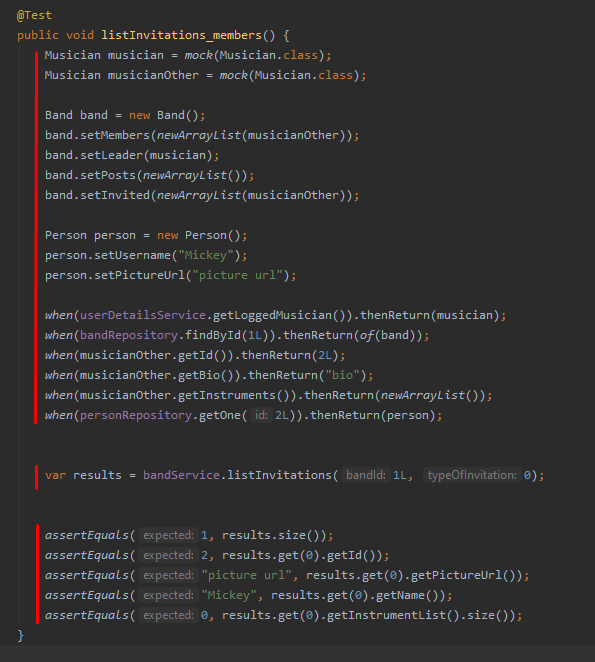
\includegraphics[width=13cm]{slike/junit_test.PNG}
				\end{center}
				\caption{Primjer JUnit testa}
				\label{fig:junit}
			\end{figure}
		
			
			Pošto je pisanje testova često i iscrpnije od pisanja implementacije (BandService ima 210 linija koda, dok BandServiceTest koji ni ne testira baš sve metode u njemu ima 558), za ovaj projekt nismo radili TDD (test driven development) već smo naknadno radili testove za postojeću implementaciju kako bismo potvrdili implementaciju i programski dokumentirali očekivano ponašanje.
			
			Uz dodatak BandService testovima postoji i nekoliko testova u EmailSenderTest koji pokazuju kako testirati komponentu čiju implementaciju ne znamo.
			
			
			Uz tridesetak JUnit testova čija je glavna prednost brzo izvođenje, napisali smo desetak integracijskih testova. Kao što smo već spomenuli, integracijski testovi slični su ručnom pregledavanju u Postmanu. Svaki integracijski test pokreće aplikaciju ispočetka tako da su mu stanje baze i aplikacije (kontekst) jednaki kao kad se pokrene aplikacija. U ovim testovima koristimo MockMvc kako bismo simulirali http request kojemu moramo odrediti metodu (GET, POST) te dodati pripadajuća zaglavlja. U ovom testu verificiramo je li ono što je vratila metoda jednako onome što se očekivalo (najčešće usporedbe DTO-ova).
			
			\begin{figure}[H]
				\begin{center}
					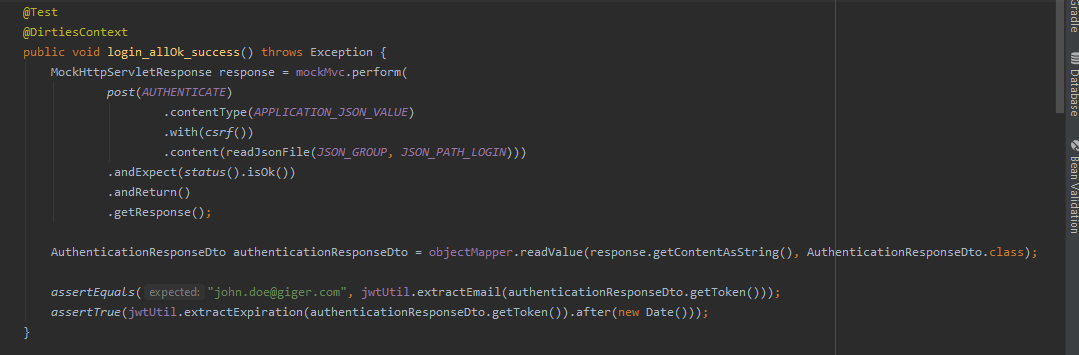
\includegraphics[width=17cm]{slike/integracijski_test.PNG}
				\end{center}
				\caption{Primjer integracijskog testa}
				\label{fig:inttest}
			\end{figure}
			
			Tehnike testiranja programske potpore nadahnute su knjigom Test-Driven Development Kenta Becka.
			
			
			
			\subsection{Ispitivanje sustava}
			
			 
		 	Za potrebe ispitivanja sustava, koristili smo Selenium IDE.
		 	
		 	\subsubsection{Test 1: Registracija korisnika}
		 		
		 		\textbf{Očekivano:} Klikom na gumb \textit{Register} otvara se forma s potrebnim poljima za registraciju: imena, prezimena, korisničkog imena, e-mail adrese, kontakt telefona te korisničke lozinke. Ukoliko su sva polja ispravna korisnik će se pokušati registrirati u bazu, u protivnom će sustav dojaviti grešku.
		 		
		 		
		 		\noindent\textbf{Rezultat:} Korisnik je uspješno registriran u bazu podataka ili je sustav dojavio grešku.\\
		 		
		 		
		 		Na slici 5.3 prikazana je poruka koja se prikaže prilikom neispravne registracije. Slika 5.4 prikazuje kako uspješna registracija izgleda u Seleniumu. U polju \textit{Value} se vide uneseni podatci za koje se testira. U \textit{Log} dijelu se vide dijelovi testa te poruka jesu li prošli ili nisu. Dok se na kraju ispiše poruka o uspješnosti testa.  
		 		
				\begin{figure}[H]
		 			\begin{center}
		 				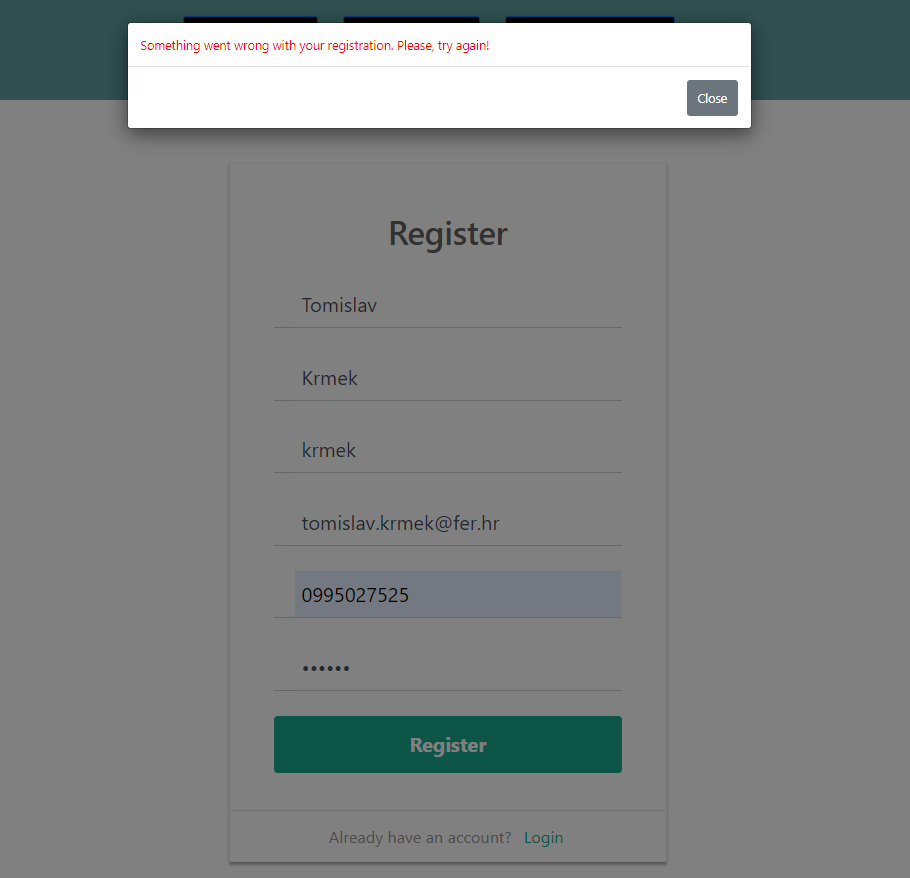
\includegraphics[width=15cm]{slike/neispravna_forma_registracija.PNG}
		 			\end{center}
		 			\caption{Prikaz poruke za neispravnu registraciju}
		 			\label{fig:inttest}
		 		\end{figure}
	 		
	 			\begin{figure}[H]
	 				\begin{center}
	 					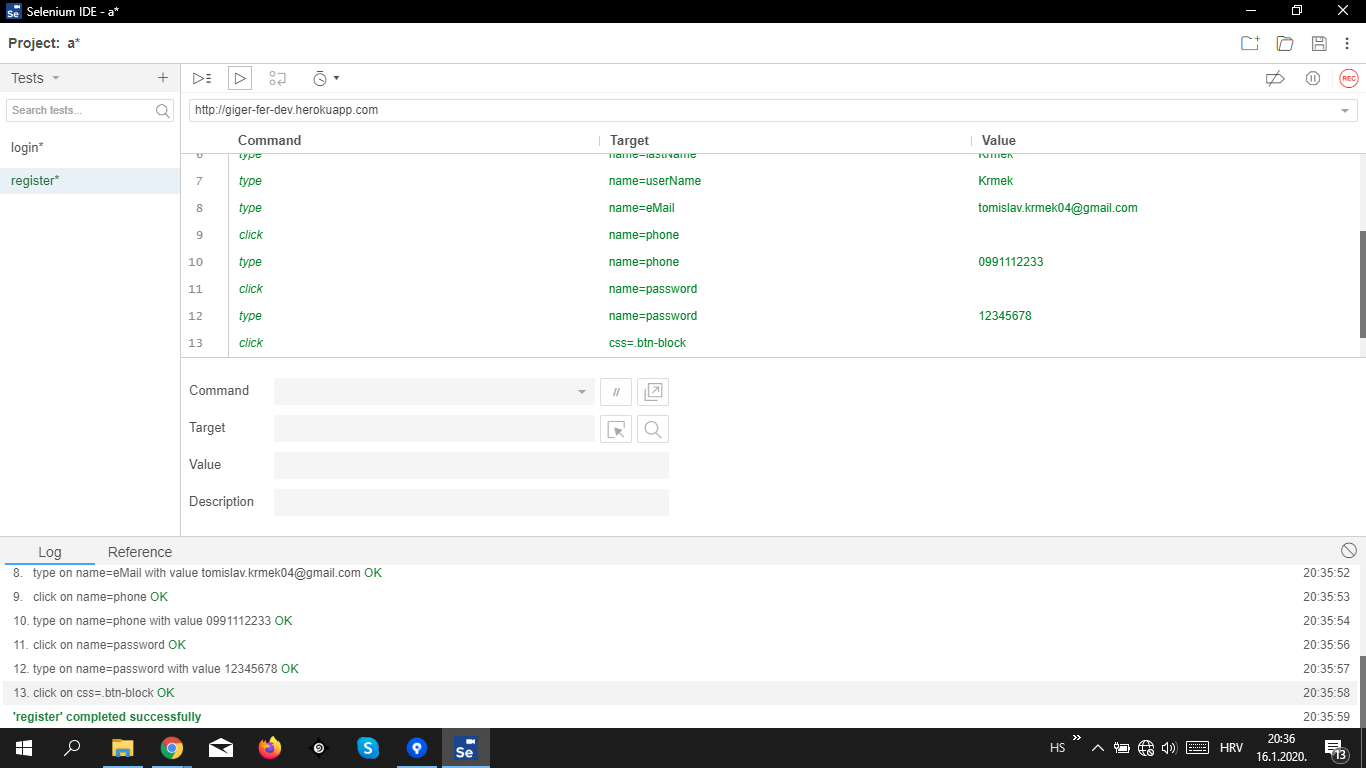
\includegraphics[width=15cm]{slike/selenium_register.PNG}
	 				\end{center}
	 				\caption{Selenium test koji prikazuje ispravnu registraciju}
	 				\label{fig:selreg}
	 			\end{figure}
 			
			\subsubsection{Test 2: Prijava korisnika u aplikaciju}
			\textbf{Očekivano:} Klikom na gumb \textit{Login} otvara se forma s poljima: e-mail korisnika i lozinka. U slučaju ispravno unešenih polja i podataka, korisnik se prijavljuje u aplikaciju. U protivnom, aplikacija dojavljuje grešku.
			
			\noindent\textbf{Rezultat:} Korisnik je prijavljen u aplikaciju ili je dojavljena greška.\\
			
			Na slici 5.5 prikazana je prijava u aplikaciju dok je na slici 5.6 prikaz javnih nastupa koji se prikaže nakon uspješne prijave. Slika 5.7 prikazuje kako to izgleda i u Seleniumu. 
			
			\begin{figure}[H]
				\begin{center}
					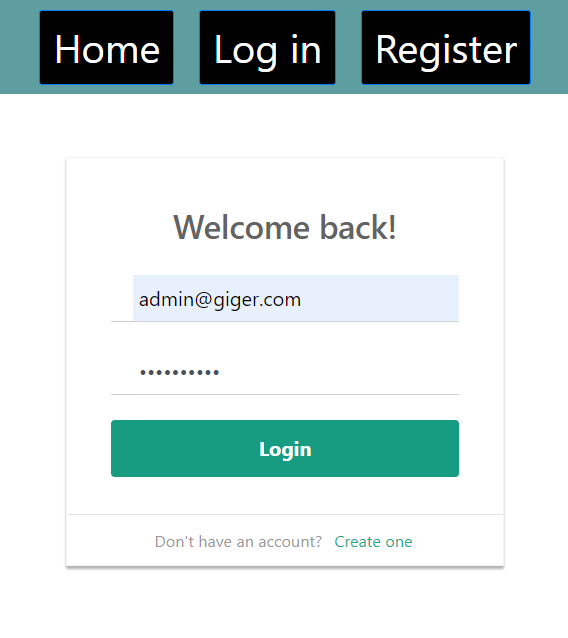
\includegraphics[width=10cm]{slike/login_screen.PNG}
				\end{center}
				\caption{Prikaz prijave u aplikaciju}
				\label{fig:login}
			\end{figure}
		
			\begin{figure}[H]
				\begin{center}
					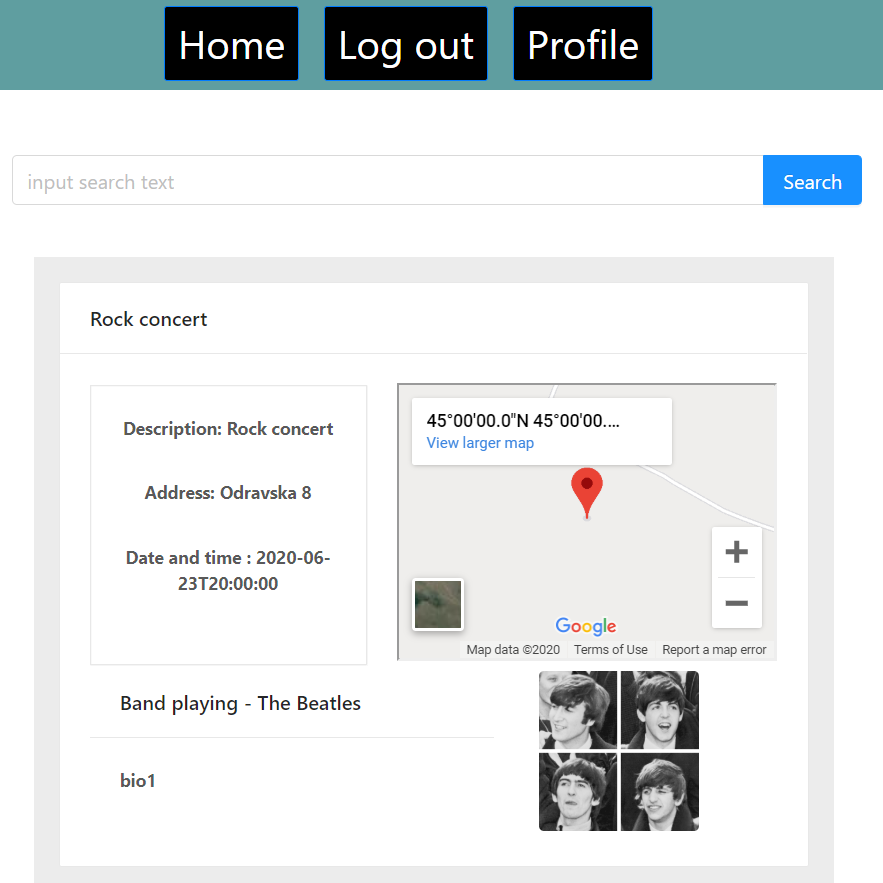
\includegraphics[width=12cm]{slike/login_redirect.PNG}
				\end{center}
				\caption{Nakon uspješne prijave, aplikacija preusmjerava na prikaz javnih nastupa}
				\label{fig:loginre}
			\end{figure}
		
			\begin{figure}[H]
				\begin{center}
					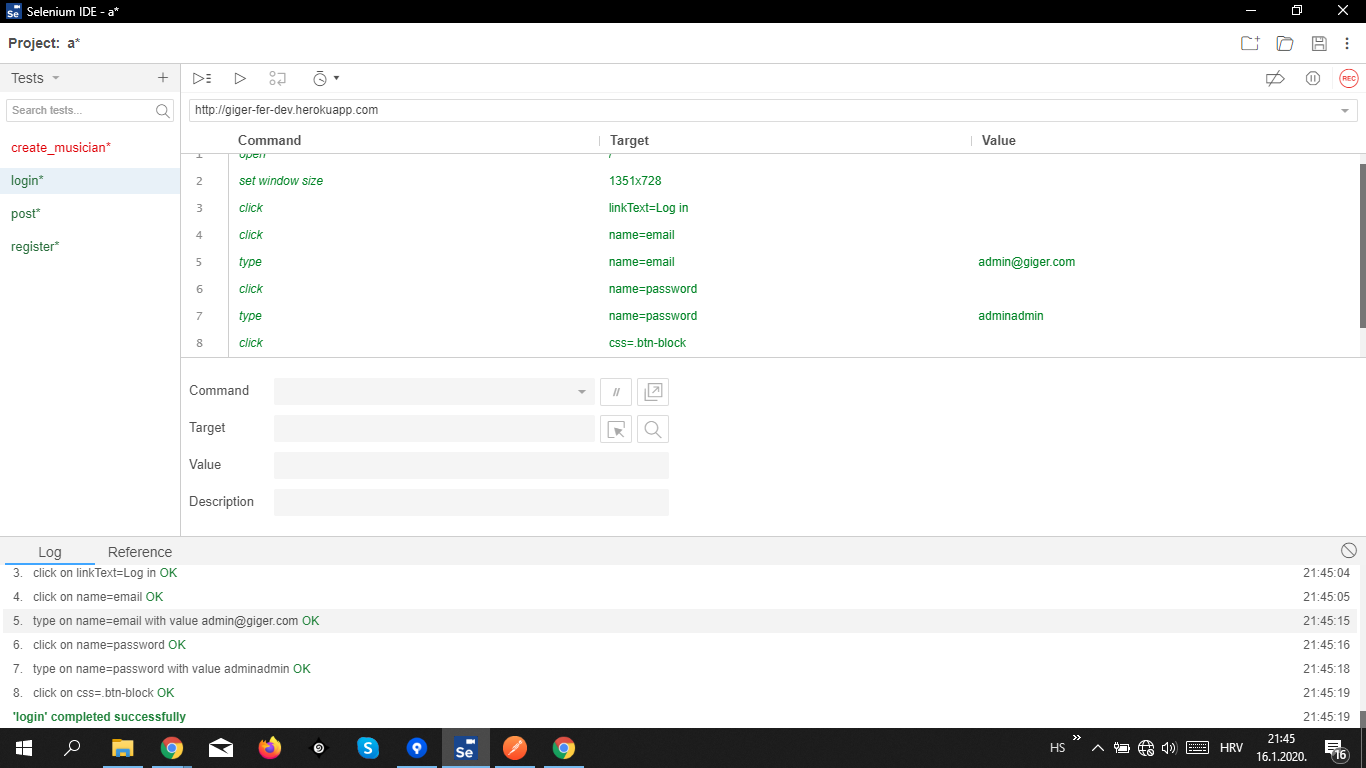
\includegraphics[width=15cm]{slike/selenium_login.PNG}
				\end{center}
				\caption{Prikaz uspješnog logina u Seleniumu}
				\label{fig:sellogin}
			\end{figure}
		
		\subsubsection{Test 3: Stvaranje profila \textit{Glazbenika}}
		\textbf{Očekivano:} Nakon prijave u aplikaciju, klikovima na gumbove: \textit{Profile, Settings, Change profile type}, nude se opcije za postati glazbenik ili organizator. Kod stvaranja organizatora je potrebno unijeti ime kao menadžera, dok kod stvaranja glazbenika je moguće unijeti biografiju, odabrati instrumente koje glazbenik svira te je li kalendar glazbenika javan ili ne. 
		\noindent Korisnik ispunjavanjem forme i klikom na gumb \textit{Confirm} stvara profil glazbenika.

		\noindent\textbf{Rezultat:} U slučaju da je korisnik već glazbenik, aplikacija će ga u pokušaju stvaranja o tome obavijestiti. U suprotnom, aplikacija dojavljuje da je korisniku uspješno dodijeljena uloga glazbenika.\\
		
		
		Na slici 5.7 prikazano je uspješno stvaranje glazbenika, dok je na slici 5.8 prikazano što se prikaže na istom mjestu u aplikaciji kada već jesmo glazbenik. Na slici 5.9 je prikazano i kako izgleda Selenium test za slučaj kada korisnik već je glazbenik. U tom slučaju, kao što vidimo, Selenium test pada.
		
		\begin{figure}[H]
			\begin{center}
				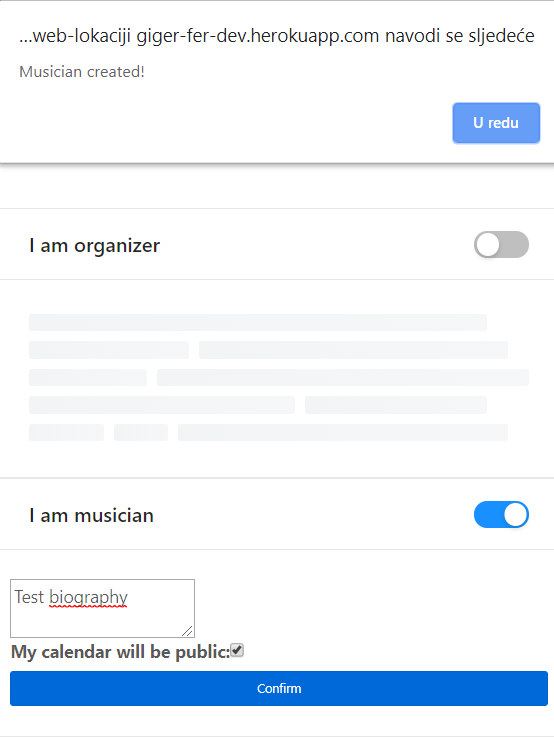
\includegraphics[width=10cm]{slike/create_musician.PNG}
			\end{center}
			\caption{Forma za stvaranje profila glazbenik}
			\label{fig:crmus}
		\end{figure}
	
		\begin{figure}[H]
			\begin{center}
				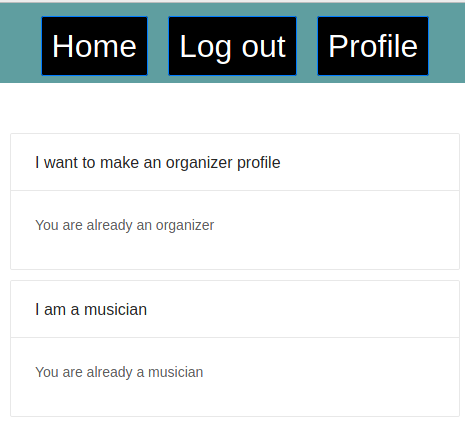
\includegraphics[width=7cm]{slike/crmus.PNG}
			\end{center}
			\caption{Forma za stvaranje profila glazbenik}
			\label{fig:crm}
		\end{figure}
	
		\begin{figure}[H]
			\begin{center}
				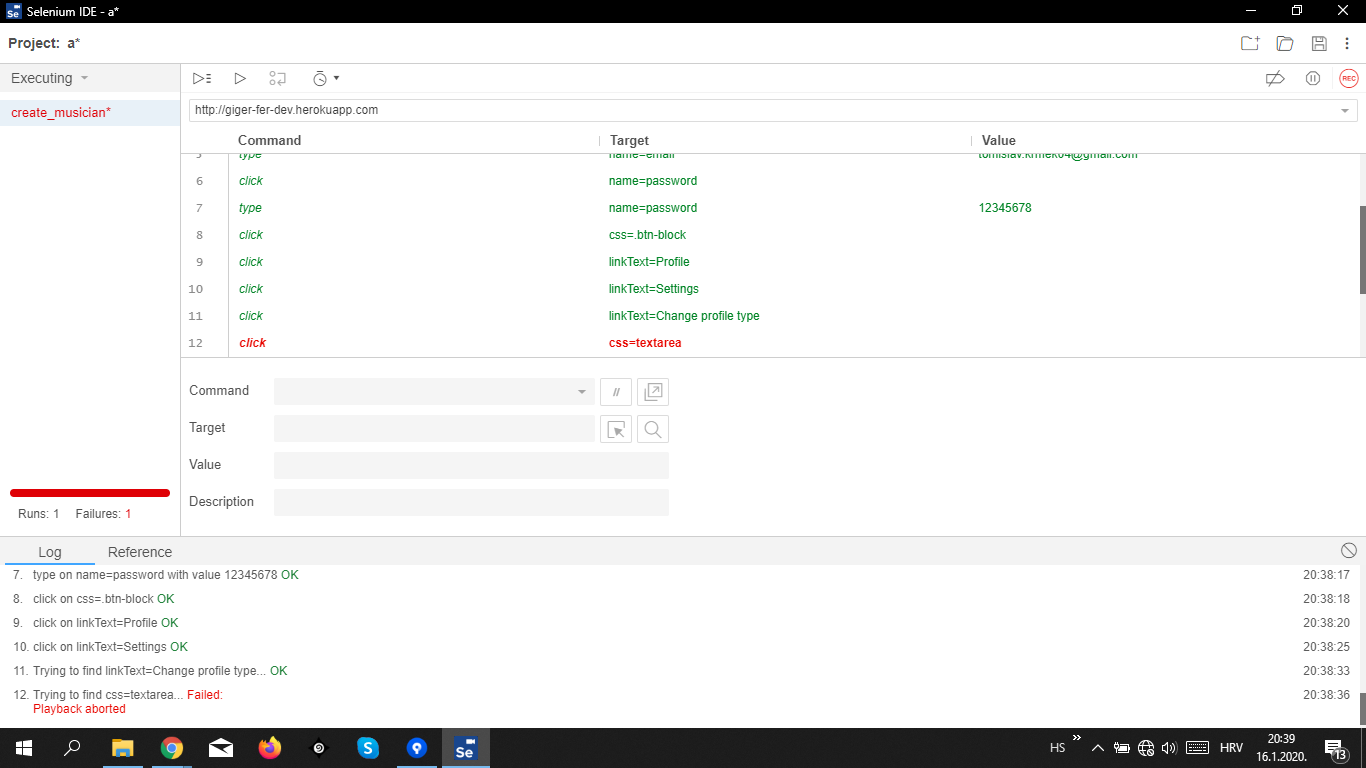
\includegraphics[width=15cm]{slike/selenium_createmus.PNG}
			\end{center}
			\caption{Prikaz Selenium testa za stvaranje profila glazbenika koji je već glazbenik}
			\label{fig:crmus2}
		\end{figure}
		
		
		\subsubsection{Test 4: Objavljivanje \textit{Post-ova}}
			\textbf{Očekivano:} Nakon što se prijavimo u aplikaciju i jesmo Glazbenik, odemo na \textit{Profile, Musician\_profile te View} gdje se prikazuju sve objave prijavljenog glazbenika. Ondje imamo i polje u koje upišemo željeni tekst objave te pritisnemo \textit{Post} kako bi se on objavio.
			
			\noindent\textbf{Rezultat:} Post se objavi i prikazuje se među ostalim objavama glazbenika.\\
			
			Na slici 5.11 je prikazano dodavanje teksta nove objave, a na 5.12 je prikazan Selenium test za dodavanje nove objave koji uspješno prođe. 
			
			\begin{figure}[H]
				\begin{center}
					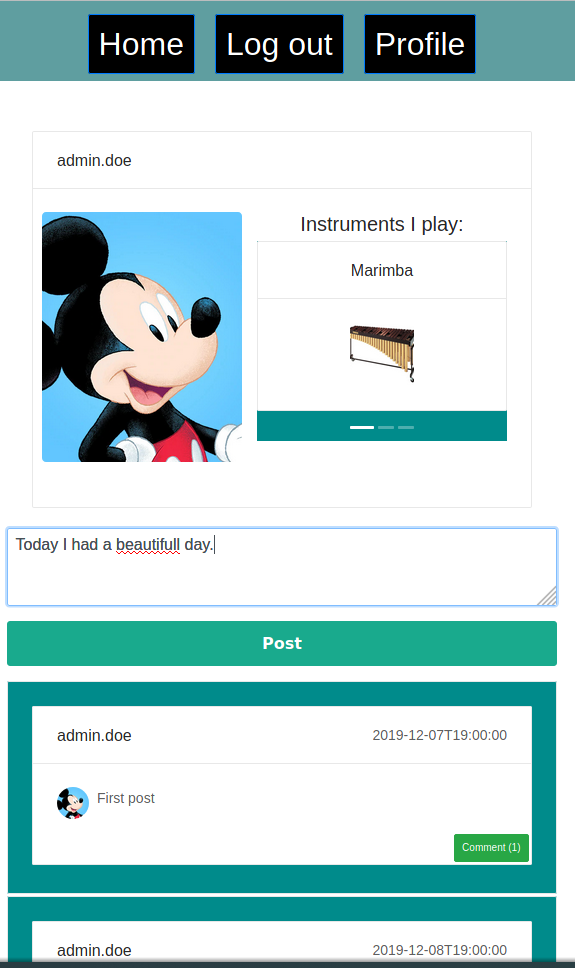
\includegraphics[width=7cm]{slike/post.PNG}
				\end{center}
				\caption{Prikaz dodavanja teksta za novu objavu}
				\label{fig:post}
			\end{figure}
		
			\begin{figure}[H]
				\begin{center}
					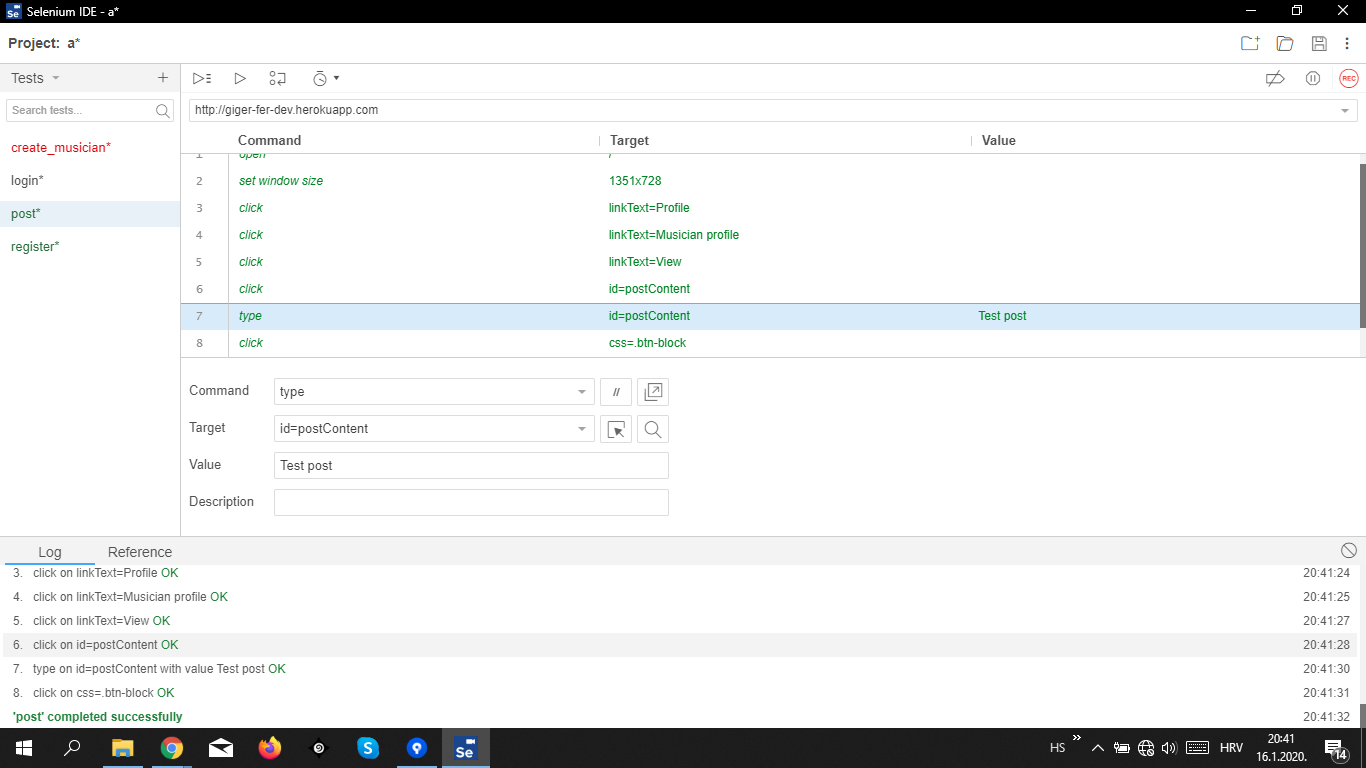
\includegraphics[width=15cm]{slike/selpost.PNG}
				\end{center}
				\caption{Prikaz Selenium testa za dodavanje objave}
				\label{fig:selpost}
			\end{figure}
			
			\eject 
		
		
		\section{Dijagram razmještaja}
			 
			 Dijagrami razmještaja opisuju topologiju sklopovlja i programsku potporu koja se koristi u implementaciji sustava u njegovom radnom okruženju. Sve komponente programske potpore smještene su na oblak platformu Heroku. Heroku kao platforma omogućuje programerima izvođenje i operiranje nad aplikacijama u oblaku. U ovome slučaju pozadinska i prednja aplikacija razmještene su na zasebene poslužitelje kao i baza podataka. Sustav je baziran na arhitekturi klijent - poslužitelj i komunikacija između njih odvija se HTTP protokolom. 
			 
			 	\begin{figure}[H]
			 	\begin{center}
			 		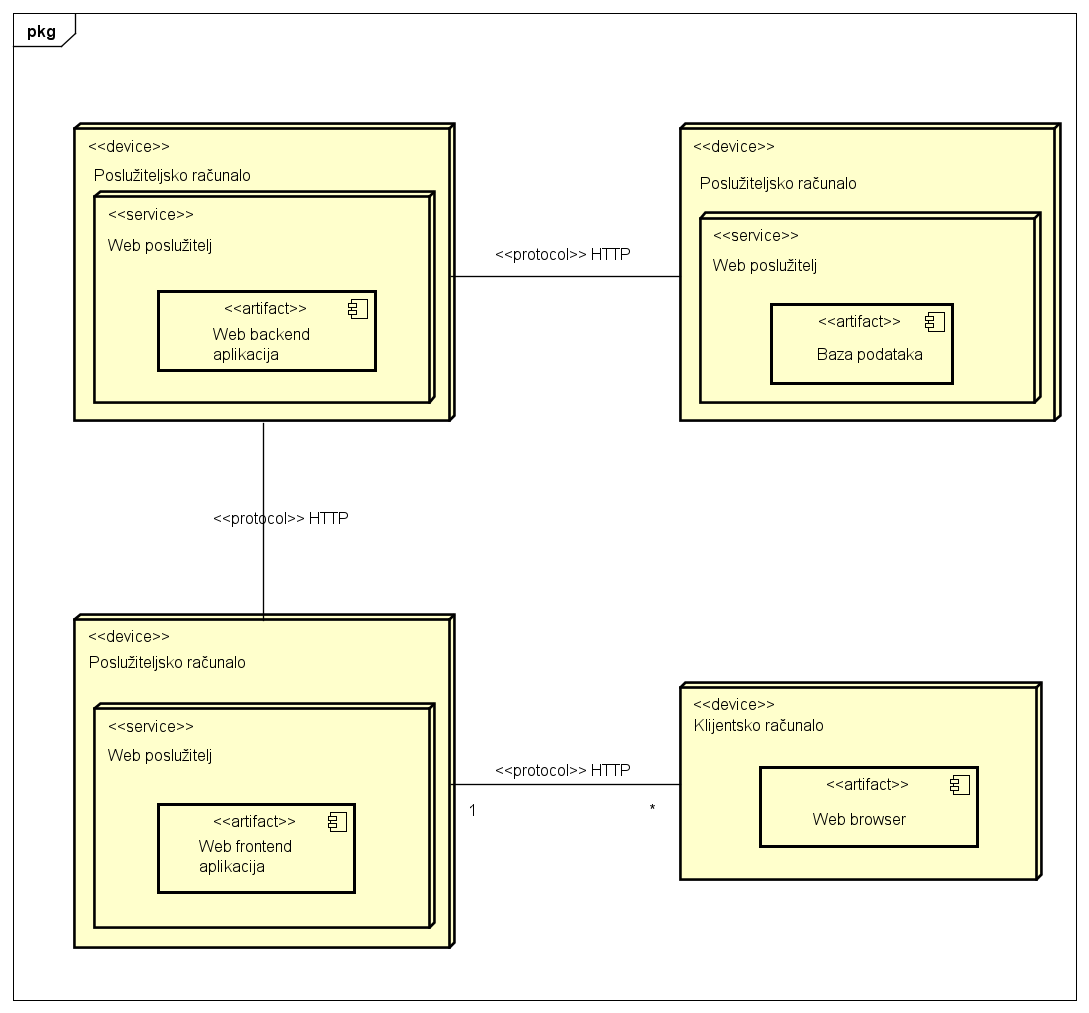
\includegraphics[width=15cm]{slike/deploy_fin.PNG}
			 	\end{center}
			 	\caption{Dijagram razmještaja}
			 	\label{fig:deploy_pic}
			 \end{figure}
			
			\eject 
		
		\section{Upute za puštanje u pogon}
			
			
			Ponajprije je potrebno preuzeti Postgres SQL bazu podataka na operacijski sustav, poželjno Windows. Nakon toga je potrebno provesti standardnu instalaciju. U servisu LoaderService nalaze se testni podaci za inicijalno punjenje baze. Za postavljanje lozinke baze potrebno je je u password polje u system-local.properties postaviti prethodno definiranu lozinku za bazu podataka. Alternativno moguće je u root direktoriju standardnog terminala  pokrenuti naredbu docker-compose up koja će u virtualnom kontejneru pokrenuti servise koji su predefinirani u dockeru docker-compose.yml datoteci. Za konfiguraciju aplikacije na Heroku poslužitelju koristi se system.properties iz kojeg se čita pokretanje Spring Boot aplikacije defaultnim profilom.
			U izradi aplikacije korišten je radni okvir Spring Boot. Za pokretanje Javine aplikacije
			potrebno je imati instaliran Java Runtime Environment v11. Za pokretanje frontend aplikacije
			potrebno je imati instaliranu platformu Node.js. Za pokretanje također je potrebno otpakirati 
			arhivu server.var. Kako bi se pokrenuo build koristi se automatizirani sustav Gradle. 
			
			\eject 